\documentclass{article}
\usepackage[utf8]{inputenc}
\usepackage{fullpage}
\usepackage{enumitem,amssymb}
\usepackage{pifont}
\usepackage{float}
\usepackage{graphicx}
\newcommand{\cmark}{\ding{51}}%
\newcommand{\xmark}{\ding{55}}%
\newcommand{\done}{\rlap{$\square$}{\raisebox{2pt}{\large\hspace{1pt}\cmark}}%
\hspace{-2.5pt}}
\usepackage{listings}
\usepackage[table,xcdraw]{xcolor}

\title{CTF header}
\author{kasperverhulst }
\date{February 2021}

\begin{document}

\begin{table}[h]
\def\arraystretch{1.8}
\begin{tabular}{|llll|}
\hline
\multicolumn{4}{|c|}{\Large \textbf{Blue}}                                                                                         \\ \hline

\multicolumn{2}{|p{0.4\textwidth}|}{Organization: TryHackMe}     &    \multicolumn{2}{|l|}{Type: VM}    \\ \hline
\multicolumn{3}{|l|}{
    \begin{minipage} [t] {0.07\textwidth} 
Categories:
    \end{minipage} 
    \begin{minipage} [t] {0.3\textwidth} 
      \begin{itemize}[label=$\square$]
            \item Network Security
            \item Cryptography
            \item Mobile Applications
            \item[\done]  Linux
     \end{itemize} 
    \end{minipage} 
     \begin{minipage} [t] {0.3\textwidth} 
      \begin{itemize}[label=$\square$]
            \item Reverse Engineering
            \item[\done] Web Applications
            \item Forensics
            \item Windows
        \end{itemize} 
    \end{minipage} } 
    & Difficulty: Easy \\ \hline 
    \multicolumn{2}{|l|}{Name: Kasper Verhulst} & 
    \multicolumn{2}{|l|}{\begin{tabular}[c]{@{}l@{}}Release date: 17-03-2019\\ Completing date: 21-04-2021 \end{tabular}} \\ \hline
\end{tabular}
\end{table}

\section{Reconnaissance}
As usual we start with an nmap scan to explore the machine

\begin{lstlisting}
$ nmap -O -sV -sC -sS -v  -oN scan.out <TARGET_IP>
\end{lstlisting} 

We see the machine is running:

\begin{table}[h]
\begin{tabular}{|l|l|l|}
\hline
\rowcolor[HTML]{9B9B9B} 
\textbf{Port} & \textbf{Service} & \textbf{Version}                                             \\ \hline
22/tcp open  & ssh            & OpenSSH 7.2p2 Ubuntu 4ubuntu2.6                                       \\ \hline
80/tcp open  & http    & Apache httpd 2.4.18                         \\ \hline
\end{tabular}
\end{table}
We can see the machine is accessible via SSH and is running an httpd webserver over HTTP. Using any CVE database, we do not find any serious vulnerabilities that currently exist to break the machine. The machine is running on Linux Ubuntu. Visit the website on http://$<$TARGET\_IP$>$:80.

\begin{figure}[H]
    
\includegraphics[width=0.7\textwidth]{index.PNG}
\end{figure}

\section{Web Enumeration}
The front page shows no links, so we can only inspect the source code. In the source code, we find commented out the username \textit{R1ckRul3s}. We try to brute force the SSH password with this username using Hydra, but apparently, the SSH connection does not allow password authentication.

\begin{lstlisting}
hydra -l R1ckRul3s -P /usr/share/wordlists/rockyou.txt  -t 4 ssh://10.10.86.145
\end{lstlisting} 

The only thing that remains us, is trying to find other web pages using a web enumeration technique like dirbuster or gobuster.

\begin{lstlisting}
gobuster dir -o gobuster-ricky.out -w /usr/share/wordlists/dirbuster/directory-list-2.3-medium.txt  -u http://10.10.86.145 -x html,php,py,txt 
\end{lstlisting}
We see there are multiple pages like portal.php, that redirect to login.php. There is also the robots.txt page where a weird string \textit{Wubbalubbadubdub} is displayed. On the login screen, we manage to login using this weird string as password and the previously found username. 

\begin{figure}[H]
    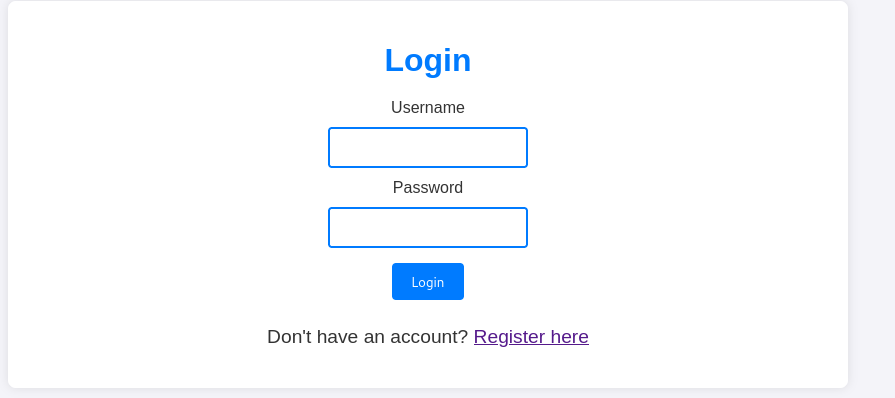
\includegraphics[width=0.7\textwidth]{login.PNG}
\end{figure}

We are now in the portal, that allows us to run commands on the web server.

\begin{figure}[H]
    \includegraphics[width=0.79\textwidth]{portal.PNG}
\end{figure}
We can see the web server is offering the files that gobuster found. Let's try to view the content of these files. For some reason, \textit{cat} and \textit{more} are blocked, but \textit{less} is not. We find the first ingredient:

\begin{lstlisting}
less Sup3rS3cretPickl3Ingred.txt
\end{lstlisting}

The clue.txt also hints us to look around on the filesystem for other ingredients. A first good idea is always to check for the users on the machine:

\begin{lstlisting}
ls /home/users
\end{lstlisting}

Here we find the second ingredient:

\begin{lstlisting}
less "/home/rick/second ingredients"
\end{lstlisting}

We don't find any other flag under /etc or similar. When you are on a machine as a non-root user, it is always a good idea to find the user's permissions. Run the command: 
\begin{lstlisting}
sudo -l
\end{lstlisting}
We see, we can run any command as root without entering a password! We find the final flag under:

\begin{lstlisting}
sudo less /root/3rd.txt
\end{lstlisting}

Note: although this machine was easy enough to enumerate and pivot through the portal interface, generally it may be a good idea to connect an interactive shell to the machine itself. For instance


\begin{enumerate}
    \item Create account or add public key for SSH access
    \item Use any of the available programming languages for reverse shell
    \item Adding a trusted account into .rhosts file
\end{enumerate}
\end{document}


